\documentclass[12pt, landscape]{article}
\usepackage[utf8]{inputenc}
\usepackage{tikz}
\usepackage{geometry}
\geometry{a4paper, margin=1in, landscape}
\usepackage{kotex} % 한글 주석을 위한 패키지

\begin{document}
\pagestyle{empty}

\begin{figure}
\centering
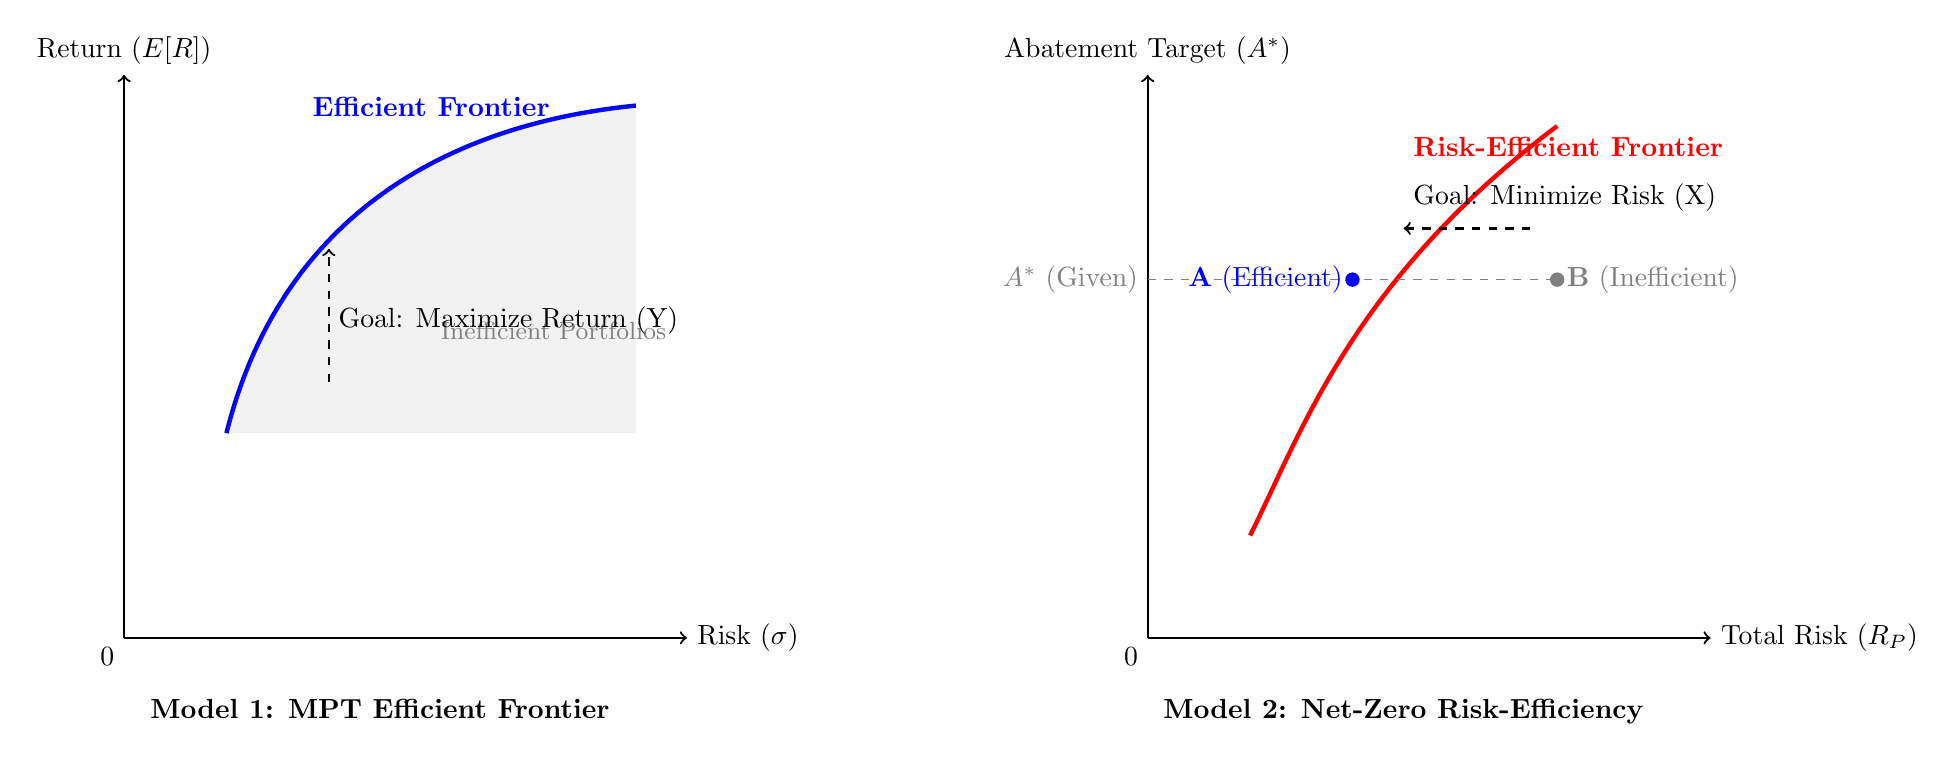
\begin{tikzpicture}[scale=1.3]
    % --- 1. MPT 그래프 ---
    \begin{scope}[xshift=-10cm]
        \draw[->, thick] (0,0) -- (5.5,0) node[right] {Risk ($\sigma$)};
        \draw[->, thick] (0,0) -- (0,5.5) node[above] {Return ($E[R]$)};
        \node[below left] at (0,0) {0};

        % MPT 효율적 투자경계 (위로 볼록)
        \draw[blue, ultra thick] (1,2) .. controls (1.5,4) and (3,5) .. (5, 5.2);
        
        % 비효율적 포트폴리오 영역
        \fill[gray, opacity=0.1] (1,2) .. controls (1.5,4) and (3,5) .. (5, 5.2) -- (5,2) -- (1,2);
        \node[gray, right] at (3, 3) {\small Inefficient Portfolios};

        % 라벨
        \node[blue, above] at (3,5) {\textbf{Efficient Frontier}};
        \node[below, align=center] at (2.5, -0.5) {\textbf{Model 1: MPT Efficient Frontier}};
        
        % 최적화 목표 설명
        \draw[->, dashed, thick] (2, 2.5) -- (2, 3.8);
        \node[right] at (2, 3.1) {Goal: Maximize Return (Y)};
    \end{scope}

    % --- 2. Net-Zero 그래프 ---
    \begin{scope}[xshift=0cm]
        \draw[->, thick] (0,0) -- (5.5,0) node[right] {Total Risk ($R_P$)};
        \draw[->, thick] (0,0) -- (0,5.5) node[above] {Abatement Target ($A^*$)};
        \node[below left] at (0,0) {0};

        % Net-Zero 위험-효율성 투자경계 (아래로 볼록)
        \draw[red, ultra thick] (1,1) .. controls (1.5,2) and (2,3.5) .. (4, 5);
        
        % 목표 지점
        \def\targetA{3.5} % 목표 A*
        \def\efficientR{2} % A 지점 R
        \def\inefficientR{4} % B 지점 R

        \draw[dashed, gray] (0, \targetA) node[left] {$A^*$ (Given)} -- (\inefficientR, \targetA);
        
        % A (효율적)
        \fill[blue] (\efficientR, \targetA) circle (2pt);
        \node[blue, left] at (\efficientR, \targetA) {\textbf{A} (Efficient)};

        % B (비효율적)
        \fill[gray] (\inefficientR, \targetA) circle (2pt);
        \node[gray, right] at (\inefficientR, \targetA) {\textbf{B} (Inefficient)};
        
        % 라벨
        \node[red, right] at (2.5, 4.8) {\textbf{Risk-Efficient Frontier}};
        \node[below, align=center] at (2.5, -0.5) {\textbf{Model 2: Net-Zero Risk-Efficiency}};

        % 최적화 목표 설명
        \draw[<-, dashed, thick] (2.5, \targetA + 0.5) -- (3.8, \targetA + 0.5);
        \node[right] at (2.5, \targetA + 0.8) {Goal: Minimize Risk (X)};
    \end{scope}

\end{tikzpicture}
\end{figure}

\end{document}
